\documentclass[tikz,border=4pt]{standalone}
\usepackage{amsmath,amssymb}
\usetikzlibrary{arrows.meta,calc,positioning,backgrounds}

\definecolor{phaseblue}{RGB}{35,105,139}
\definecolor{phaseorange}{RGB}{189,89,43}
\definecolor{ink}{RGB}{40,42,46}
\definecolor{softgray}{RGB}{238,239,241}
\definecolor{midgray}{RGB}{145,149,156}

\begin{document}
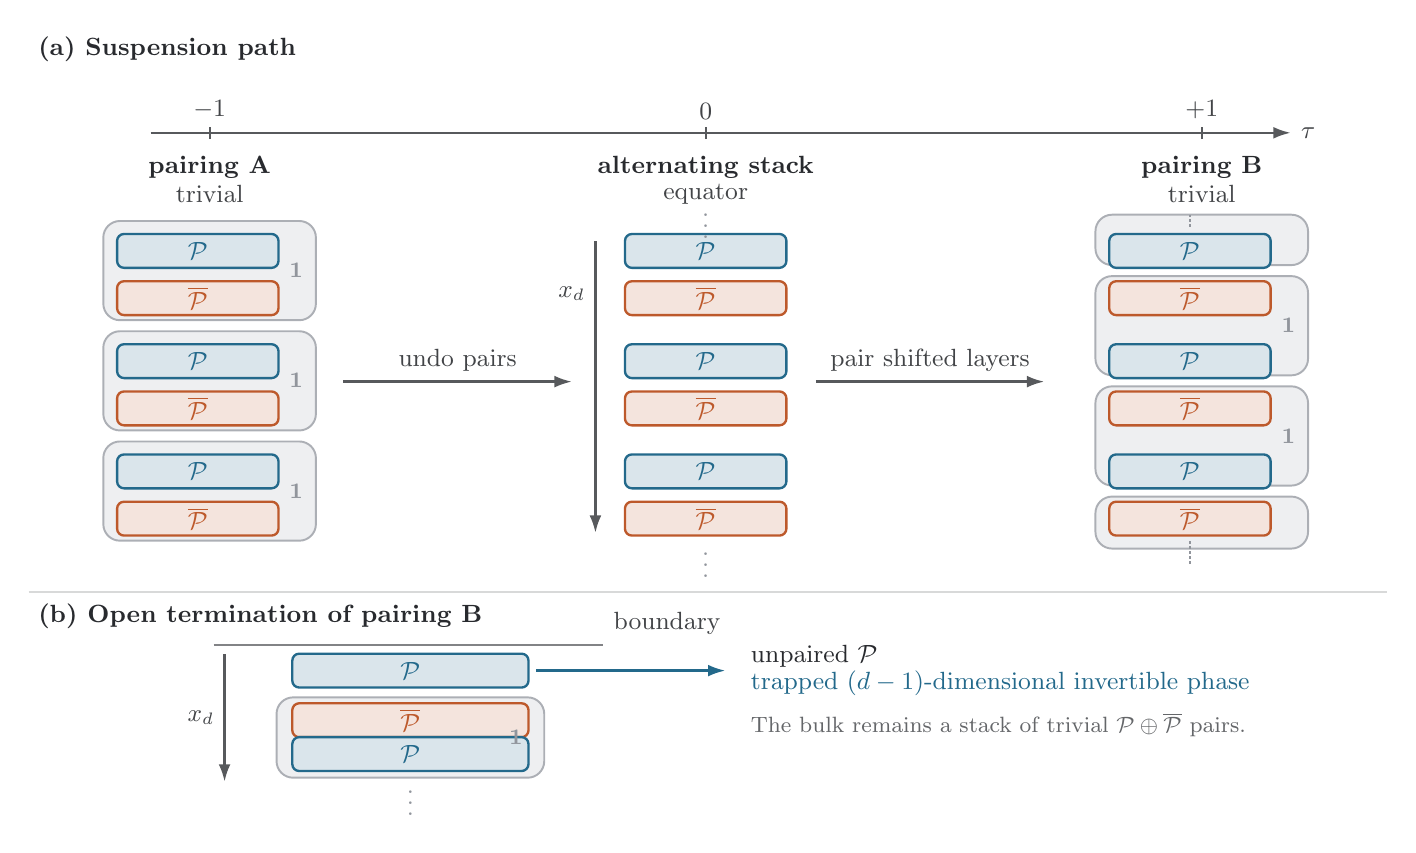
\begin{tikzpicture}[
  x=1cm,y=1cm,
  font=\small,
  phase/.style={rounded corners=2.5pt,minimum width=2.05cm,
                minimum height=.43cm,line width=.85pt,inner sep=1pt},
  p/.style={phase,draw=phaseblue,fill=phaseblue!17,text=phaseblue},
  pinv/.style={phase,draw=phaseorange,fill=phaseorange!16,text=phaseorange},
  pairbox/.style={rounded corners=6pt,draw=midgray!75,fill=softgray,
                 line width=.7pt},
  flow/.style={-{Latex[length=2.2mm,width=1.5mm]},draw=ink!78,line width=.85pt},
  return/.style={-{Latex[length=2.2mm,width=1.5mm]},draw=midgray,
                 densely dashed,line width=.8pt},
  note/.style={text=ink!88,align=center},
  title/.style={text=ink,font=\small\bfseries}
]

% Panel (a): the suspension path.
\node[anchor=west,title] at (.15,8.92) {(a) Suspension path};

% Suspension coordinate.
\draw[flow] (1.70,7.86)--(16.18,7.86)
  node[right,note] {$\tau$};
\foreach \xx/\lab in {2.45/-1,8.75/0,15.05/{+1}}{
  \draw[ink!78,line width=.75pt] (\xx,7.78)--(\xx,7.94);
  \node[above,note] at (\xx,7.91) {$\lab$};
}

% First contraction.
\node[title] at (2.45,7.42) {pairing A};
\node[note] at (2.45,7.08) {trivial};
\begin{scope}[on background layer]
  \draw[pairbox] (1.10,5.48) rectangle (3.80,6.74);
  \draw[pairbox] (1.10,4.08) rectangle (3.80,5.34);
  \draw[pairbox] (1.10,2.68) rectangle (3.80,3.94);
\end{scope}
\node[p]    at (2.30,6.36) {$\mathcal P$};
\node[pinv] at (2.30,5.76) {$\overline{\mathcal P}$};
\node[p]    at (2.30,4.96) {$\mathcal P$};
\node[pinv] at (2.30,4.36) {$\overline{\mathcal P}$};
\node[p]    at (2.30,3.56) {$\mathcal P$};
\node[pinv] at (2.30,2.96) {$\overline{\mathcal P}$};
\node[text=midgray,font=\footnotesize] at (3.55,6.11) {$\mathbf 1$};
\node[text=midgray,font=\footnotesize] at (3.55,4.71) {$\mathbf 1$};
\node[text=midgray,font=\footnotesize] at (3.55,3.31) {$\mathbf 1$};

% Alternating stack at the equator.
\node[title] at (8.75,7.42) {alternating stack};
\node[note] at (8.75,7.08) {equator};
\node[p]    at (8.75,6.36) {$\mathcal P$};
\node[pinv] at (8.75,5.76) {$\overline{\mathcal P}$};
\node[p]    at (8.75,4.96) {$\mathcal P$};
\node[pinv] at (8.75,4.36) {$\overline{\mathcal P}$};
\node[p]    at (8.75,3.56) {$\mathcal P$};
\node[pinv] at (8.75,2.96) {$\overline{\mathcal P}$};
\node[text=midgray] at (8.75,6.78) {$\vdots$};
\node[text=midgray] at (8.75,2.47) {$\vdots$};
\draw[flow] (7.35,6.48)--(7.35,2.78)
  node[pos=.18,left,note] {$x_d$};

% Shifted contraction.  The partial boxes indicate continuation of the
% infinite/periodic bulk stack.
\node[title] at (15.05,7.42) {pairing B};
\node[note] at (15.05,7.08) {trivial};
\begin{scope}[on background layer]
  \draw[pairbox] (13.70,4.78) rectangle (16.40,6.04);
  \draw[pairbox] (13.70,3.38) rectangle (16.40,4.64);
  \draw[pairbox] (13.70,6.18) rectangle (16.40,6.82);
  \draw[pairbox] (13.70,2.58) rectangle (16.40,3.24);
\end{scope}
\node[p]    at (14.90,6.36) {$\mathcal P$};
\node[pinv] at (14.90,5.76) {$\overline{\mathcal P}$};
\node[p]    at (14.90,4.96) {$\mathcal P$};
\node[pinv] at (14.90,4.36) {$\overline{\mathcal P}$};
\node[p]    at (14.90,3.56) {$\mathcal P$};
\node[pinv] at (14.90,2.96) {$\overline{\mathcal P}$};
\node[text=midgray,font=\footnotesize] at (16.15,5.41) {$\mathbf 1$};
\node[text=midgray,font=\footnotesize] at (16.15,4.01) {$\mathbf 1$};
\draw[midgray,densely dotted,line width=.8pt] (14.90,6.67)--(14.90,6.82);
\draw[midgray,densely dotted,line width=.8pt] (14.90,2.67)--(14.90,2.38);

% Flow through the two contractions.
\draw[flow] (4.15,4.70)--(7.05,4.70)
 node[midway,above,note] {undo pairs};
\draw[flow] (10.15,4.70)--(13.05,4.70)
 node[midway,above,note] {pair shifted layers};
% Divider.
\draw[ink!18,line width=.6pt] (.15,2.03)--(17.40,2.03);

% Panel (b): boundary consequence.
\node[anchor=west,title] at (.15,1.72) {(b) Open termination of pairing B};
\draw[ink!58,line width=.75pt] (2.50,1.36)--(7.45,1.36)
  node[above right,note] {boundary};
\draw[flow] (2.64,1.24)--(2.64,-.38)
  node[midway,left,note] {$x_d$};

\begin{scope}[on background layer]
  \draw[pairbox] (3.30,-.33) rectangle (6.70,.69);
\end{scope}
\node[p,minimum width=3.0cm]    at (5.00,1.03) {$\mathcal P$};
\node[pinv,minimum width=3.0cm] at (5.00,.40) {$\overline{\mathcal P}$};
\node[p,minimum width=3.0cm]    at (5.00,-.03) {$\mathcal P$};
\node[text=midgray,font=\footnotesize] at (6.34,.18) {$\mathbf 1$};
\node[text=midgray] at (5.00,-.55) {$\vdots$};

\draw[flow,phaseblue] (6.60,1.03)--(9.00,1.03);
\node[anchor=west,align=left,text=ink] at (9.20,1.03)
  {unpaired $\mathcal P$\\[-1pt]
   \textcolor{phaseblue}{trapped $(d-1)$-dimensional invertible phase}};
\node[anchor=west,align=left,text=ink!72,font=\footnotesize] at (9.20,.34)
  {The bulk remains a stack of trivial $\mathcal P\oplus\overline{\mathcal P}$ pairs.};

\end{tikzpicture}
\end{document}
